% Encapsulation of one CHUNK_REQ (R5): cap1 frame 317. TikZ fragment, \input by
% report/sections/05-capture.tex. Sizes from tshark: frame.len 154, eth 14, ip.hdr_len 20,
% tcp.hdr_len 32, meshsync header 12, body_len 76 (88 TCP payload, 120 segment, 140 packet).
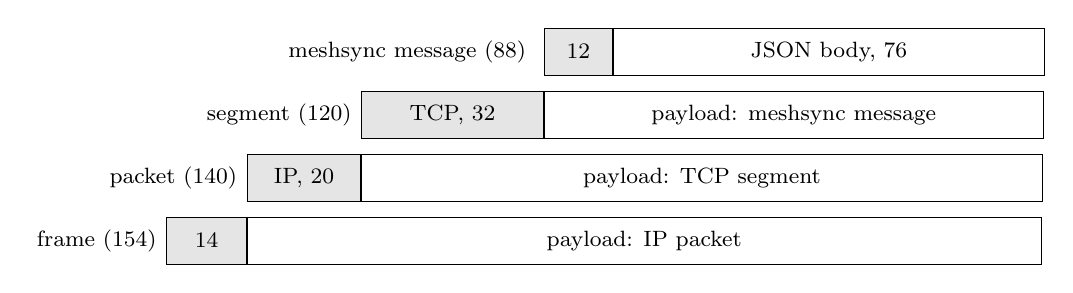
\begin{tikzpicture}[font=\footnotesize, box/.style={draw, minimum height=6mm, inner sep=2pt},
    hd/.style={box, fill=black!10}, pl/.style={box, fill=white}]
  \def\u{0.072} % cm per byte
  % row 4: application message
  \node[hd, minimum width=12*\u cm, anchor=west] (mh) at (6.6,0) {12};
  \node[pl, minimum width=76*\u cm, anchor=west] (mb) at (mh.east) {JSON body, 76};
  \node[anchor=east] at (6.5,0) {meshsync message (88)};
  % row 3: TCP segment
  \node[hd, minimum width=32*\u cm, anchor=east] (th) at (6.6,-0.8) {TCP, 32};
  \node[pl, minimum width=88*\u cm, anchor=west] (tp) at (th.east) {payload: meshsync message};
  \node[anchor=east] at (th.west) {segment (120)};
  % row 2: IP packet
  \node[hd, minimum width=20*\u cm, anchor=east] (ih) at (th.west |- 0,-1.6) {IP, 20};
  \node[pl, minimum width=120*\u cm, anchor=west] (ip) at (ih.east) {payload: TCP segment};
  \node[anchor=east] at (ih.west) {packet (140)};
  % row 1: frame
  \node[hd, minimum width=14*\u cm, anchor=east] (fh) at (ih.west |- 0,-2.4) {14};
  \node[pl, minimum width=140*\u cm, anchor=west] (fp) at (fh.east) {payload: IP packet};
  \node[anchor=east] at (fh.west) {frame (154)};
\end{tikzpicture}
